\documentclass[tikz,border=2pt]{standalone}
\usepackage{tkz-euclide}

\begin{document}
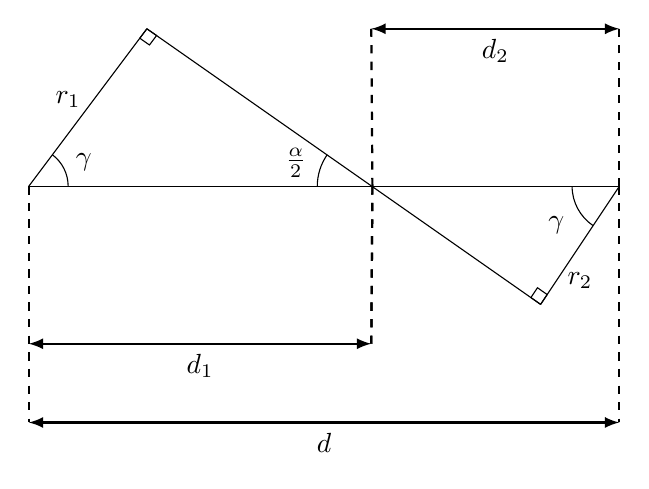
\begin{tikzpicture}

  % Centers and crossing point
  \tkzDefPoints{0/0/O1, 7.5/0/O2, 4.364/0/P}

  \tkzDefPoint(1.5, 2){T1top}
  \tkzDefPoint(6.5,-1.5){T2bot}

  % Cross tangent lines (extended)
  \draw (T1top) -- (T2bot);

  % Radii to tangent points
  \draw (O1) -- (T1top);
  \draw (O2) -- (T2bot);

  % Horizontal line of centers
  \draw (O1) -- (O2);

  % Angle gamma at O1
  \tkzMarkAngle[size=0.5](P,O1,T1top)

  % Angle gamma at O2
  \tkzMarkAngle[size=0.6](P,O2,T2bot)

  % Angle alpha at crossing pint P
  \tkzMarkAngle[size=0.7](T1top,P,O1)

  \tkzMarkRightAngle[size=0.15](P,T1top,O1)
  \tkzMarkRightAngle[size=0.15](P,T2bot,O2)

  \draw [thick, dashed] (O1) -- (0,-3);
  \draw [thick, dashed] (P) -- (4.35,2);
  \draw [thick, dashed] (O2) -- (7.5,2);

  \draw [thick, dashed] (O2) -- (7.5,-3);
  \draw [thick, dashed] (P) -- (4.35,-2);
  \draw [thick, dashed] (P) -- (4.35,-2);

  \draw[latex-latex, thick] (0,-2) -- (4.35,-2) node[midway, below] {$d_1$};
  \draw[latex-latex, thick] (4.35,2) -- (7.5,2) node[midway, below] {$d_2$};
  \draw[latex-latex, thick] (0,-3) -- (7.5,-3) node[midway, below] {$d$};

  % Labels
  \node at (0.5, 1.1)  {$r_1$};
  \node at (0.7,  0.3) {$\gamma$};
  \node at (7, -1.2)  {$r_2$};
  \node at (6.7,  -0.5) {$\gamma$};
  \node[fill=white, inner sep=2pt, rounded corners=2pt] at (3.39,
  0.3)  {$\frac{\alpha}{2}$};

\end{tikzpicture}
\end{document}
